\documentclass[fignum,nobf,man]{apa}
\usepackage{apacite}
\usepackage{bm}
\usepackage{pcl}
\usepackage{graphicx}
\usepackage{mathtools}
\usepackage[longnamesfirst]{natbib}
\usepackage[american]{babel}
\usepackage{setspace} 

\rightheader{Dominance, Power, and Constraint}
\shorttitle{Dominance, Power, and Constraint}

\leftheader{Rouder \& Haaf}

\author{Jeffrey N. Rouder \& Julia M. Haaf}

\title{Dominance, Power, and Constraint: A note on the appeal of within-subject designs.}

\affiliation{University of Missouri}

\note{\begin{flushleft}

\vspace{1in}
Jeff Rouder\\
rouderj@missouri.edu\\
Word Count:
\end{flushleft}
}

\abstract{Yup
}

\acknowledgements{Email: rouderj@missouri.edu, Web: pcl.missouri.edu; Twitter: @JeffRouder.}  

\begin{document}
\maketitle



%\renewenvironment{knitrout}{\begin{singlespace}}{\end{singlespace}}

The practice of psychological science is going through a period of rapid transition where methodological concerns are front and center.  One longstanding, salient concern is that too many experiments are underpowered (citations).   There are two consequences of underpowered designs.  First, if a design is underpowered, then, at least from a classical point-of-view, there is an increased chance of failing to detect an effect.  When this failure happens, the interpretation is muddied as it is unclear if such failures reflect a lack of power or a truly null effect.  Second, and perhaps more perniciously, 

One solution to the problem of underpowered designs is simply to add more participants.  Indeed, informally, we have observed several rules of thumb.    We examine here the wisdom of the requisite-minima advise for cognitive psychologists.  


One reason to think it is overstated comes from psychophysics and perceptual psychology.  Experiments in this domain have provided some of the clearest and most persuasive insights.  Examples include, ..., (use the Yantis book).  Yet, in contradiction to the requisite-minima advise, almost all psychophysical experiments use a small number of participants.  One of our favorite examples is XX---not only are there three participants, the participants have the same initials as the authors.  The first author has published twice experiments with only three people \citep{Ratcliff:Rouder:1998,Rouder:etal:2005}.  We contend tha

The {\em psychophysical design tradition} may be described by three properties:  1. The use of very small numbers of participants; 2. the use of within-subject manipulations; and 3. the use of ver large numbers of trials per participant.  This tradition may be compared to two other traditions.  In the {\em cognitive design tradition} there are usually a moderate number of participants, say 20, a mix of within-subject and between-subject manipulations, and moderate numbers of trials per participants, say from 10 to 100.  The other pole are social-psychological and survey designs where there are a great many participants, often between-subject designs, and a single if not handful of observations per participant.  It is our observation that social psychologists have been the most vocal about requisite minima advise, and have been the most energetic in meeting these minima. 

For this paper, we restrict our attention to understanding power in within-participant designs.  We ask how the trade-off between numbers of trials per participant and number of participants should be made.  Take, for example, whether 4 participants should run 250 trials per condition, whether 10 participants should run 100 trials per condition, whether 100 participants should run 10 trials per condition, or whether 250 participants should run 4 trials per condition.  As a practical concern, it would be preferred if we could obtain reasonable power with the fewest participants running the most trials.  The reason is straightforward---the marginal cost of adding more trials to an experiment is always less than adding more participants.   Once the participants are in the lab, it takes only 30 minutes or so to perform a few hundred trials in many cognitive and perceptual tasks.  Therefore, fewer participants mean less time and money spent getting data.

\section{}
It is our observation that many psychologist think of statistics as a set of procedures than may be applied to data of a certain type or in a certain design.  In this procedural view, statistics take the 
Suppose that participants provide response times to two conditions, generically called {\em treatment} and {\em control}.  Examples might be a priming experiments where primed and unprimed stimuli comprise the treatment and control condition, respectively.  We assume that each participant performs a large number of trials in each condition.  Let $Y_{ijk}$ denote the $k$th replicate, $k=1,\ldots,K$, for the $i$th participant, $i=1,\ldots,I$ in the $j$th condition, $j=1,2$ for control and treatment, respectively. 

The usual course of analysis is to aggregated across replicate to produce $\bar{Y}_{ij}$, a participant-by-condition mean RT.  Then, these are submitted to a paired $t$-test.  In the paired t-test, the difference, $d_i$, the participant's observed effect given by $d_i=\bar{Y}_{i2}-\bar{Y}_{i2}$, is modeled as a normal, .e.g, 
\begin{eqa}
d_i \sim \mbox{Normal}(\mu_d,\sigma^2_d)
\end{eqa}  
The question answered is whether the data are discordant with the supposition that $\mu_d=0$.  The $t$-statistic in this case is 
\[
t=\frac{\sqrt{I}\times\bar{d}}{s_d},
\]
where $\bar{d}$ and $s_d$ are the mean and standard deviation, respectively, of the observed participant effects, $d_1,\ldots,d_I$.  The $t$-value increases with increasing number of participants, increasing mean effects, and decreasing variability across these effects.  Increasing the number of participants has an obvious effect; increasing $K$, the number of observations.  

The distribution of the $t$ statistic is known in this case:
\[
t\sim\mbox{T}(I-1,\frac{\sqrt{I}\mu_d}{\sigma_d}),
\]
where the first argument $I-1$ is the familiar degrees of freedom, and the second argument, $\sqrt{I}\mu_d/\sigma_d$, is known as the noncentrality parameters.  The larger the noncentrality parameter, the more powerful the test.  Figure~\ref{power-v-ncp} shows the relationship for a few values of $I$.

\begin{figure}
\includegraphics[width=3.5in]{power-v-ncp.pdf}
\caption{Power as a function of the noncentrality parameter of a t-test.}
\label{power-v-ncp}
\end{figure}

It is helpful to consider a model on the observations themselves rather than the observed difference:
 With this, we may model $Y_{ijk}$ as
\begin{eq}\label{dataMod}
Y_{ijk} \sim  \mbox{Normal}(\mu_{ij},\sigma^2).
\end{eq}
We refer to $\sigma^2$ as {\em trial noise}---it is the variability across replicate trials from the same condition for the same participant.  It is the noise that cannot be reduced or decomposed.

The cell means $\mu_{ij}$ can be expressed as:
\begin{eqa*}
\mu_{i1} &=& \mu_i-\alpha_i/2\\
\mu_{i2} &=& \mu_i+\alpha_i/2\\
\end{eqa*}
Here $\mu_i$ is a participant-specific overall grand-mean latency across both conditions; $\alpha_i$ is the participant specific effect.    We assume here both $\mu_i$ and $\alpha_i$, e.g., $\mu_i \sim \mbox{Normal}(\nu_\mu,\delta_\mu)$ and $\alpha_i\mbox{Normal}(\nu_\alpha,\delta_\alpha)$.   The term $\delta_\alpha$ is called the {\em population noise}---it is how variable true effects are across the population.  


With these assumptions, $\bar{Y}_{i1} \sim \mbox{Normal}(\mu_i+\alpha_i/2,\sigma^2/K)$ and $\bar{Y}_{i2} \sim \mbox{Normal}(\mu_i+\alpha_i/2,\sigma^2/K)$.  The difference, $d_i$ is distributed as $d_i|\alpha_i \sim \mbox{Normal}(\alpha_i,2\sigma^2/K)$.  Marginalizing this random variable across  $\alpha_i$ yields 
\[
d_i \sim \mbox{Normal}(\nu_\alpha,\delta_\alpha+2\sigma^2/K).
\]

The resulting $t$ value is distributed as
\[
t\sim\mbox{T}(I-1,\frac{\sqrt{I}\nu_\alpha}{\sqrt{\delta_\alpha+2\sigma^2/K}}).
\]
The critical quantity, the noncentrality parameter, is 
\[
\lambda=\frac{\sqrt{I}\nu_\alpha}{\sqrt{\delta_\alpha+2\sigma^2/K}}.
\]
After some rearrangement, the noncentrality can be expressed as
\begin{eqa} \label{noncentrality}
\lambda = \sqrt{\nu_\alpha^2 \times  \frac{IK}{K\delta_\alpha+2\sigma^2}}.
\end{eqa}

From Eq. (\ref{noncentrality}), it is clear that increasing the number of people, $I$, is always results in greater power than increasing the number of replicates, $K$.   The reason is that although $I$ and $K$ enter into the numerator, $K$ also enters into the denominator.  Hence, noncentral must increase at a greater rate with $I$ than $K$.

The effectiveness of increasing $K$ depends on the amount of trial noise and population noise.  When population noise is relatively small, that is all people have a similarly sized effect, then increasing $K$ is much as increasing $I$.  This behavior is shown in Figure~\ref{tradeoff}A.  Here, power is plotted for a range of $I$ and $K$.  Of course, as both $I$ and $K$ increase, power increases.  The critical question is about trading $I$ for $K$.  The points show power for $I\times K=1000$ for different values.  These points form an iso-sample-size power curve, and as can be seen, although it is better to have large numbers of people and smaller numbers of trials per participant, the effect is not large.  For the shown curves, the far left point at $K=10$ ($I=100$) has power of .82 while the far right point at $K=100$ ($I=10$) has a power of .60.  This difference in power entails the massive inconvenience of recruiting 100 rather than 10 participants.  If 80\% power is desired, there are many choices that are practically better than $I=100$ and $K=10$.  For example, this power level may be obtained for 15 participants at 100 trials per condition.  Note that although such a design entails  far fewer participants than recommended by requisite minima, the power is exceedingly high.  We feel such a choice is judicious as resources are not wasted recruiting excessive numbers of participants.  


\begin{figure}
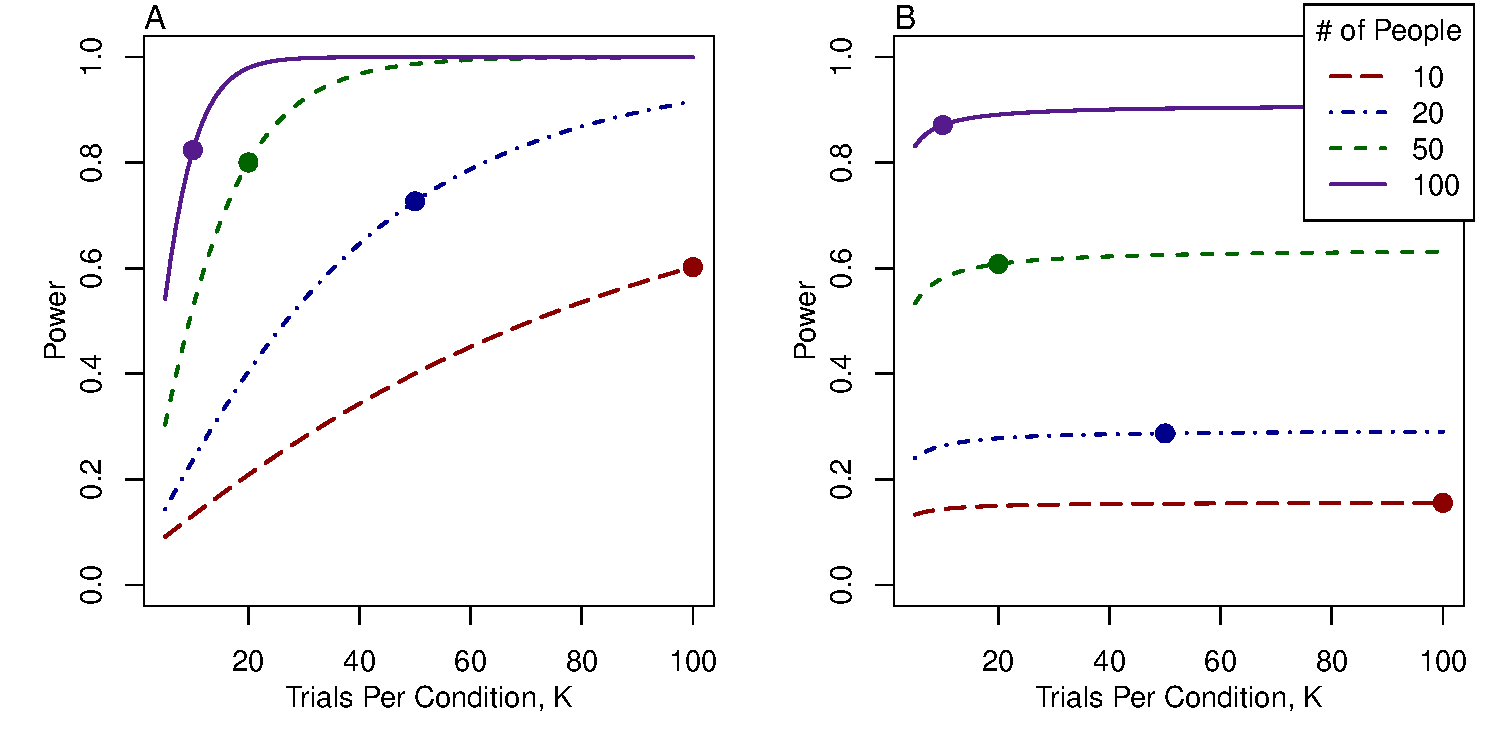
\includegraphics[width=7in]{tradeoff.pdf}
\caption{Power as a function of $I$, the number of participants, and $K$, the number of observations per condition per person.  {\bf A}.  Population noise is small relative to trial noise ($\sqrt{\delta_\alpha}=$28 ms, $\sigma=$300 ms).  {\bf B}.  Population noise is large relative to trial noise ($\sqrt{\delta_\alpha}=$120 ms, $\sigma=$100 ms). }
\label{tradeoff}
\end{figure}


In the above case, trial noise was relatively large compared to population noise.  Consider the reverse where population noise is relatively large compared to trial noise.  In this case, increasing $K$ is largely ineffective as it enters into both the numerator and denominator.  Figure~\ref{tradeoff}B shows the power curves.   These curves flatten for large $K$ indicating the only way to beat population noise is to increase the number of participants.  Shown also is the iso-sample-size power curve which shows the strong advantage for designs with large numbers of participants.


\section{Dominance in Action}
The critical question then to researchers is the relation among population noise and trials noise.  If population noise is small, then high power may be obtained by increasing the number of replicates.  Conversely, if population noise is large, then the only route to high power is the more expensive and less attractive designs with large numbers of participants.

We think the former case almost always holds.  Trial noise in our view is most often the limiting factor, and consequently, we believe researchers can often increase their power without hassle by increasing the numbers of replicate trials.  

The argument starts with consideration of the nature of individual differences.  While individual differences in Stroop effects, memory, or perception are expected, it is reasonable to suspect there are certain dominance constraints that are obeyed.  In the Stroop task, for example, it is reasonable to expect that all individuals truly read congruent items at least as fast as incongruent ones, and that no individual truly reads incongruent items faster than congruent ones.  Likewise, for all individuals, the identification of bright flashes is truly better than dim ones, and memory for oft-repeated items is truly better than once-presented items.   Of course, in any finite sample we may observe reversals by chance; the supposition is that the true values do not reverse.

Figure shows distributions of true effects that do and do not obey dominance.  Indominant distributions of effects, such as the normal, imply that some people have truly positive effects while others have truly negative effects.  The dominance setup we explore is the one on the right.  Here, there are a few distributions corresponding to different sized effects.  For example, the first curve shows a small effect, the next a medium effect, and the last a large effect.  Note how the variance increases with the mean.  In some sense, this pattern has to hold.  If effects are constrained to be positive and small, then the variance must be small as well. 

Let's consider a Stroop task .  The trial noise in the time to name color words is roughly around 300 ms in standard deviation.  If we suspect there is dominance, then Stroop effects might reasonably distributed as the middle curve in xx.  This curve has a mean of 40 ms and a standard deviation of 28 ms.    These values are those used in drawing Figure XX, and as can be seen, high power may be achieved with as few as 10 or 15 participants so long as there are sufficient trials per condition.  

\section{Discussion}

In this paper we have argued that requisite-minima advise on the numbers of participants in an experiment may be short sided.  Our main point was that a constellation of factors, the mean effect, the trial noise, the population noise, and, importantly, the number of trials per condition all contribute to power.  The relationship is not overly complex, and high power with small numbers of participants is achievable when the population noise is relatively small compared to the trial noise.

We have argued that indeed small values of population is to be expected based on a dominance principle.  We suspect that nobody Stroops backwards or responds faster to weaker stimuli.  And if dominance holds, then the relatively small effects we typically mine must be associated with small true population noise as well.  If the noise was bigger, either the effect would need to be greater or dominance would be violated.  




\end{document}
